
\documentclass[]{article}
\usepackage{emptypage}
\usepackage{subcaption}
\usepackage{graphicx}
\title{Investigating Individual Differences in Structural MRI on Human Connectom Project Dataset\\ Search Light Analysis }
\author{NAHAR}

\begin{document}
%1) Categorical RSA (running)
%2) PCA on left and right thickness, and their cross-color plots
%3) Multivariate and univariate searchlight maps for left and right thickness
%4) Multiclass SVM with libsvm
%5) Pairwise RDM model and other RDM models
%6) Categorical and non-categorical RSA for thickness left and right
\maketitle
\thispagestyle{empty}
\pagenumbering{arabic}

\newpage

\section{ Curvature Left RSA}
\centerline{\includegraphics[width=0.8\textwidth]{RSAModels_Curvature_Left.png}}
\centerline{\includegraphics[width=0.8\textwidth]{RSAHists_Curvature_Left.png}}
\centerline{\includegraphics[width=1\textwidth]{RSAMaps_Curvature_Left.png}}
\newpage
\vspace*{-3cm}
\section{Curvature Right RSA}
\centerline{\includegraphics[width=0.7\textwidth]{RSAModels_Curvature_Right.png}}
\centerline{\includegraphics[width=0.7\textwidth]{RSAHists_Curvature_Right.png}}
\centerline{\includegraphics[width=.9\textwidth]{RSAMaps_Curvature_Right.png}}

\newpage
\vspace*{-3cm}
\section{PCA Representations}
\centerline{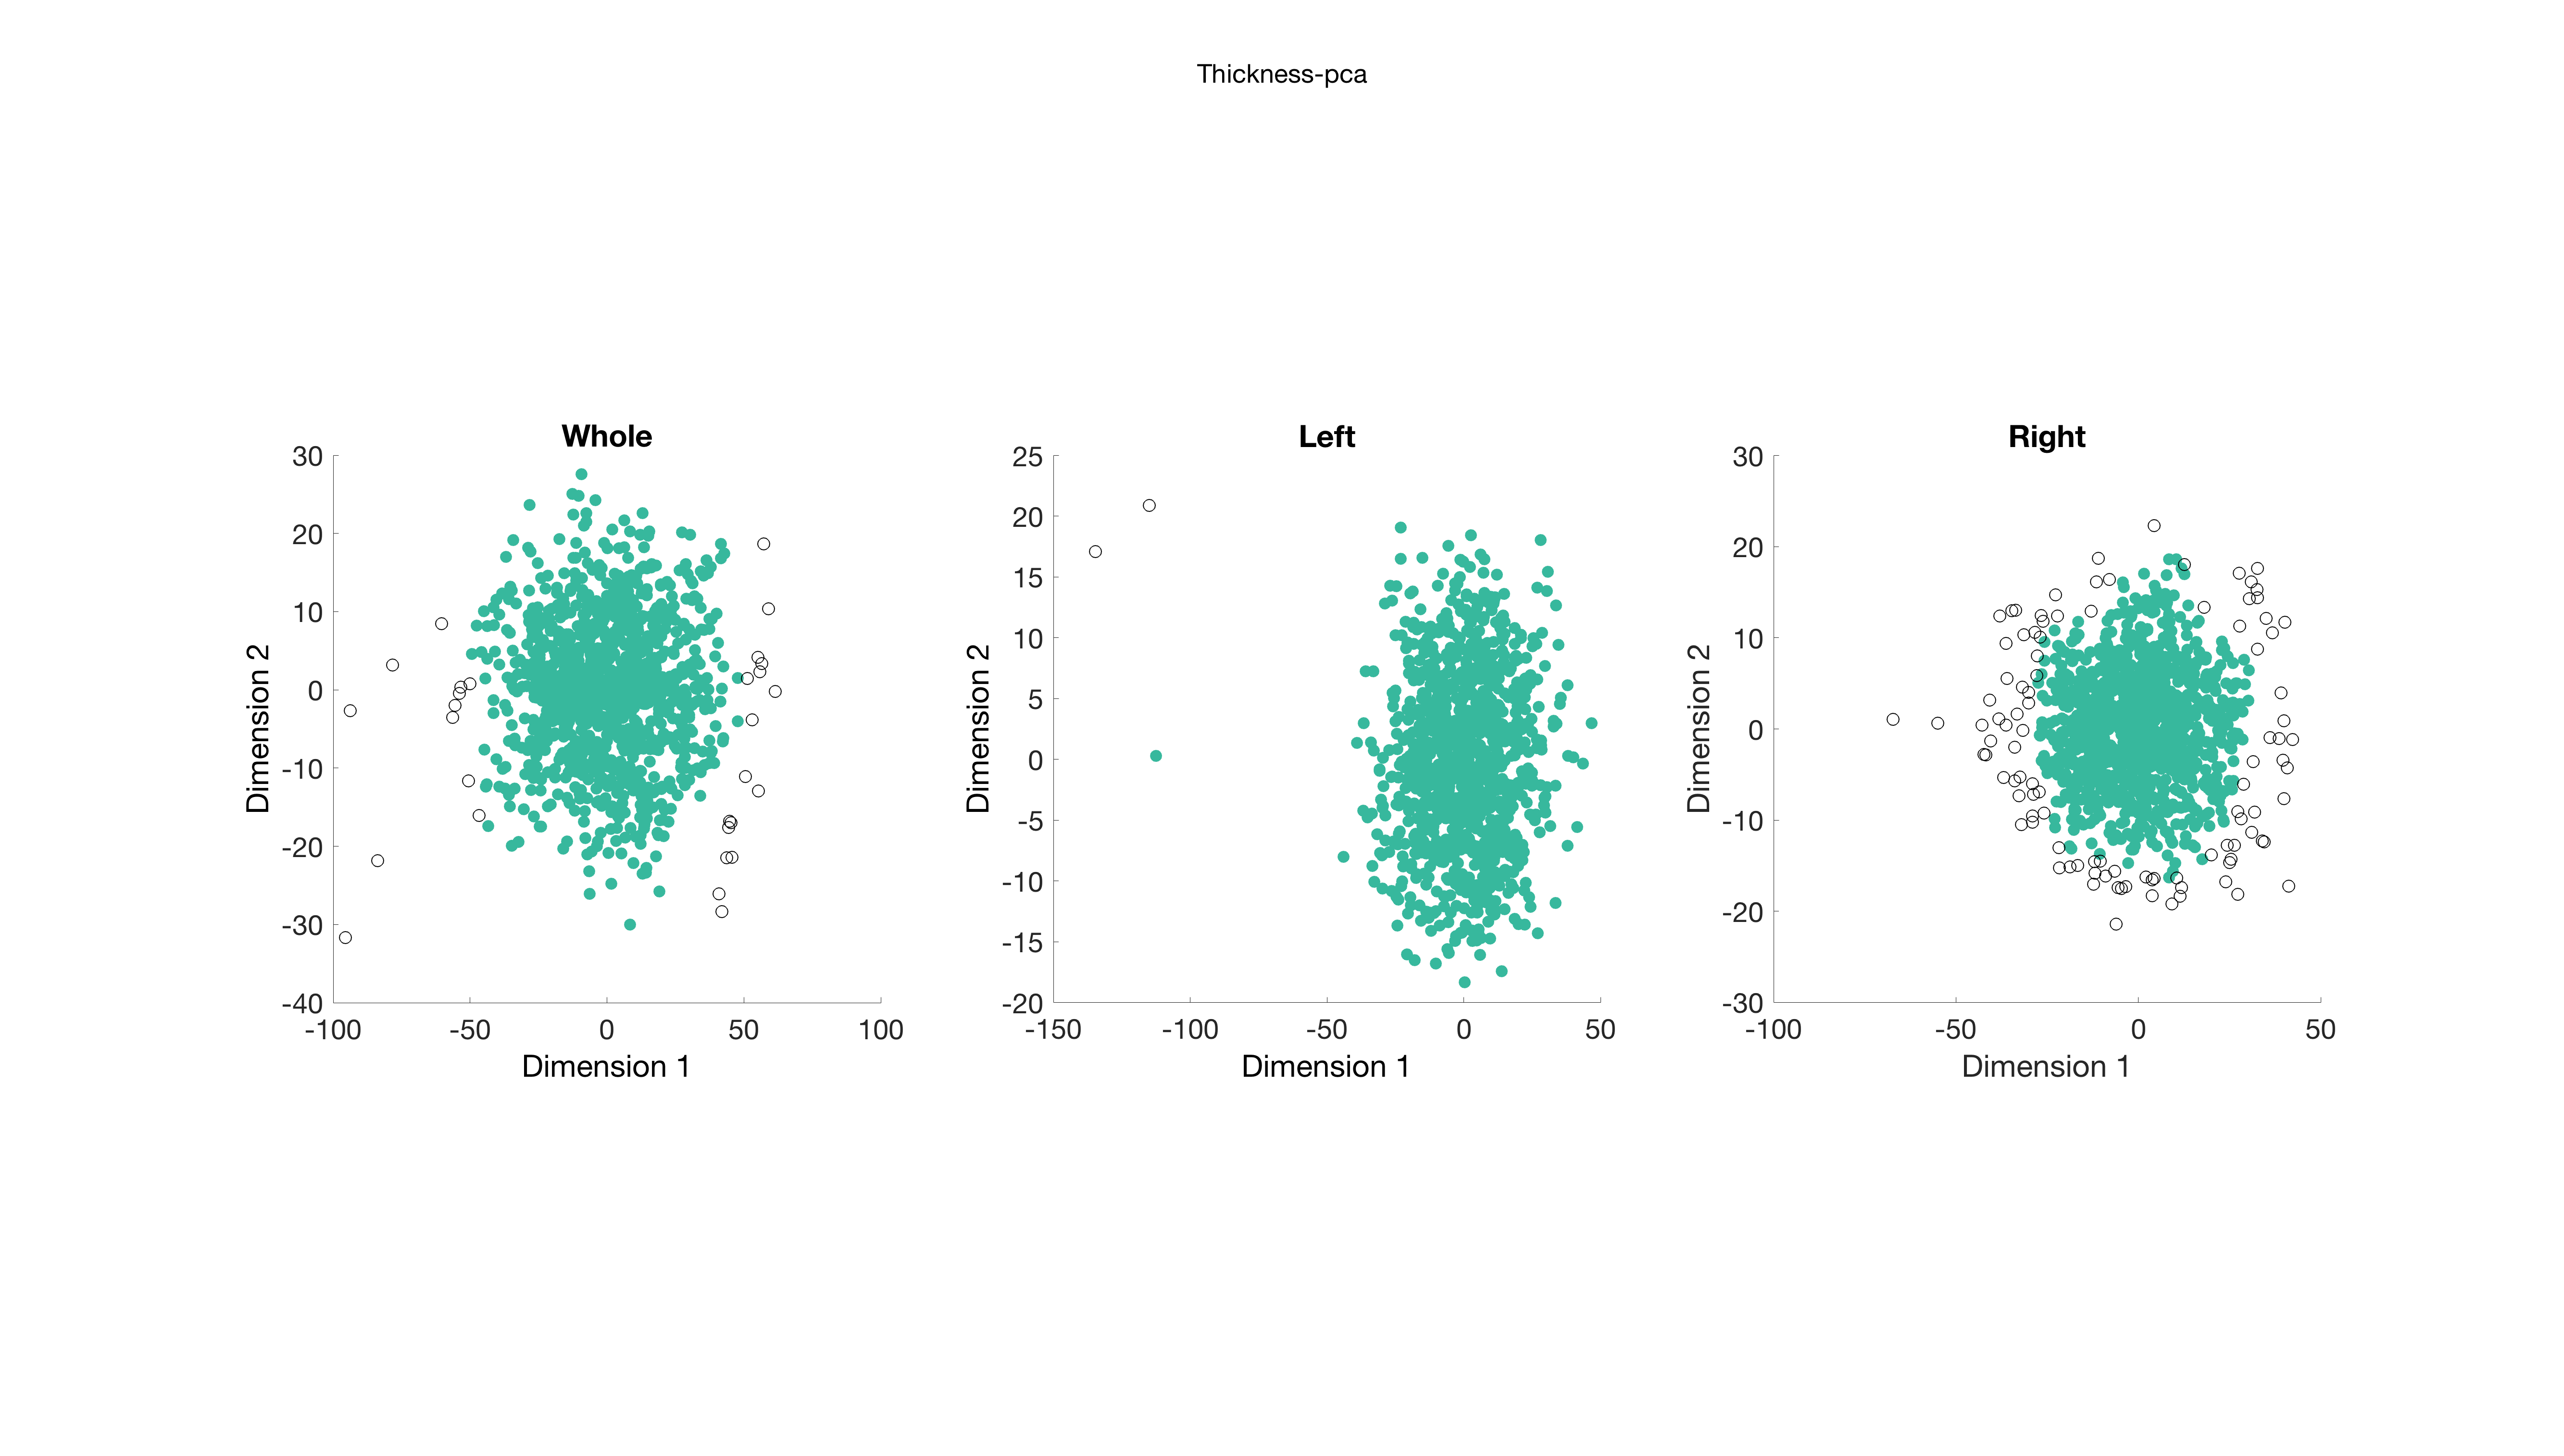
\includegraphics[width=1\textwidth]{LowDReps_Thickness_pca.png}}
\vspace*{-1cm}
\centerline{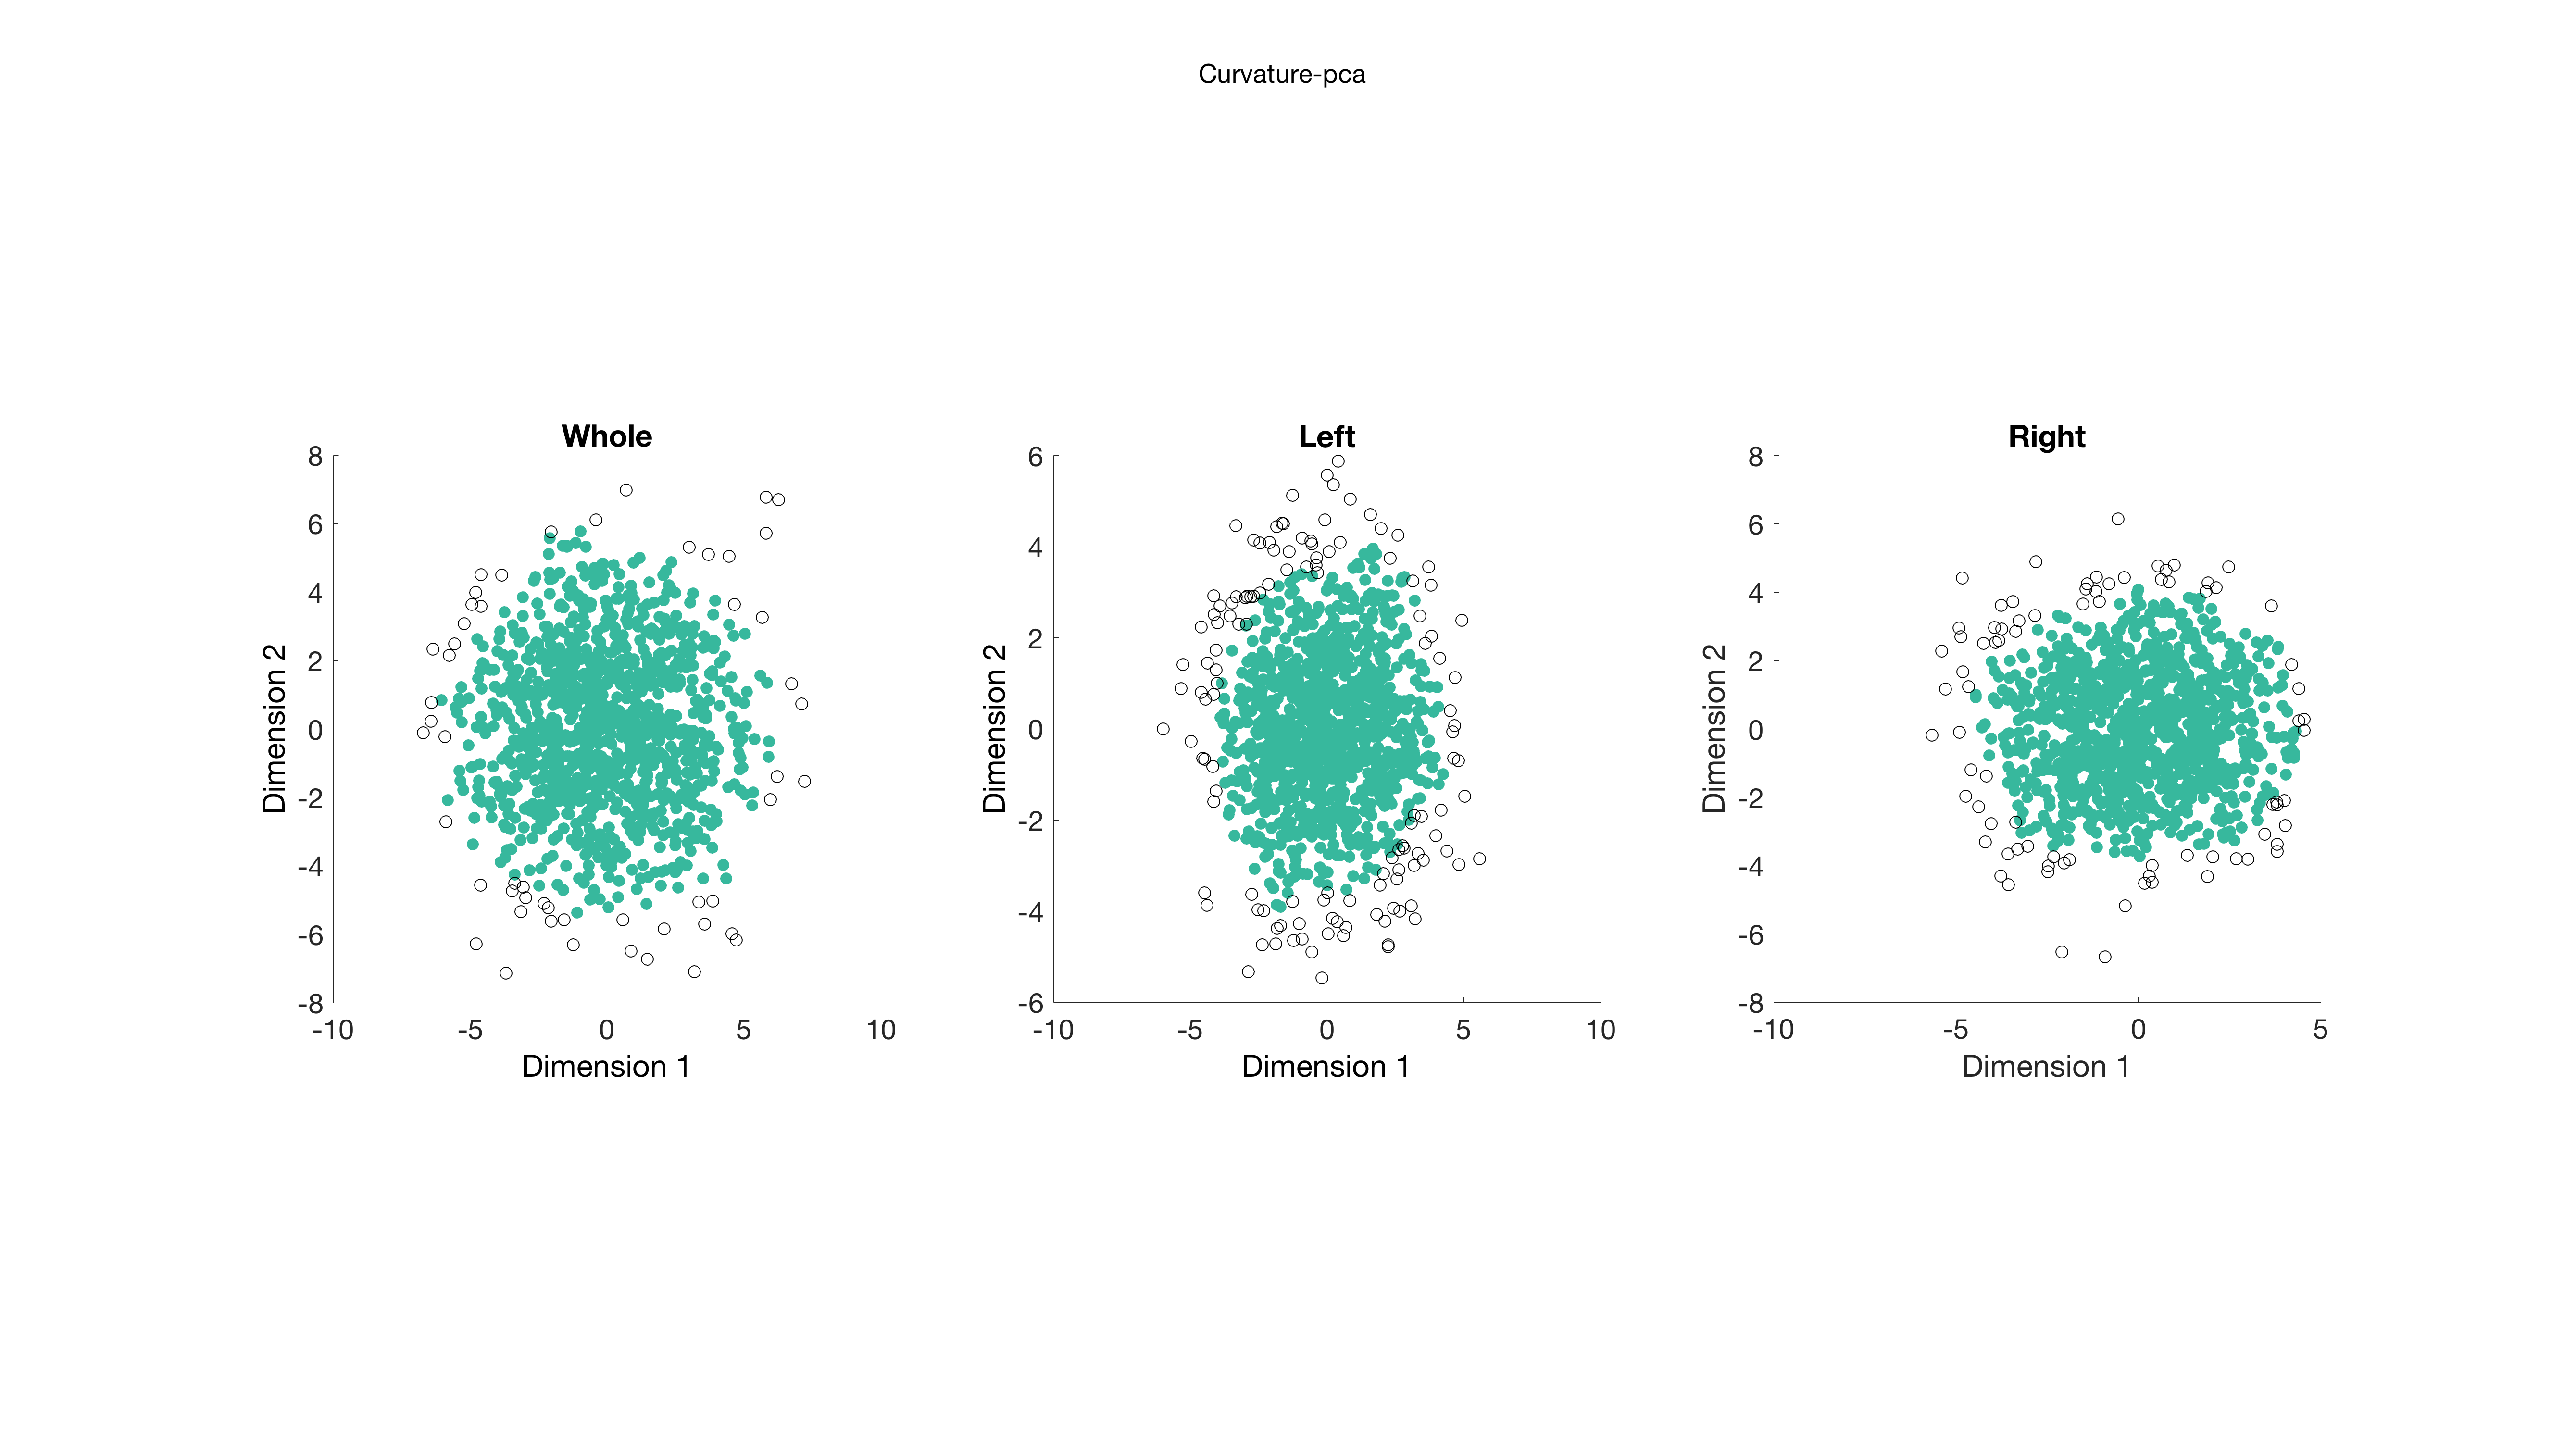
\includegraphics[width=1\textwidth]{LowDReps_Curvature_pca.png}}
\vspace*{-1cm}
\centerline{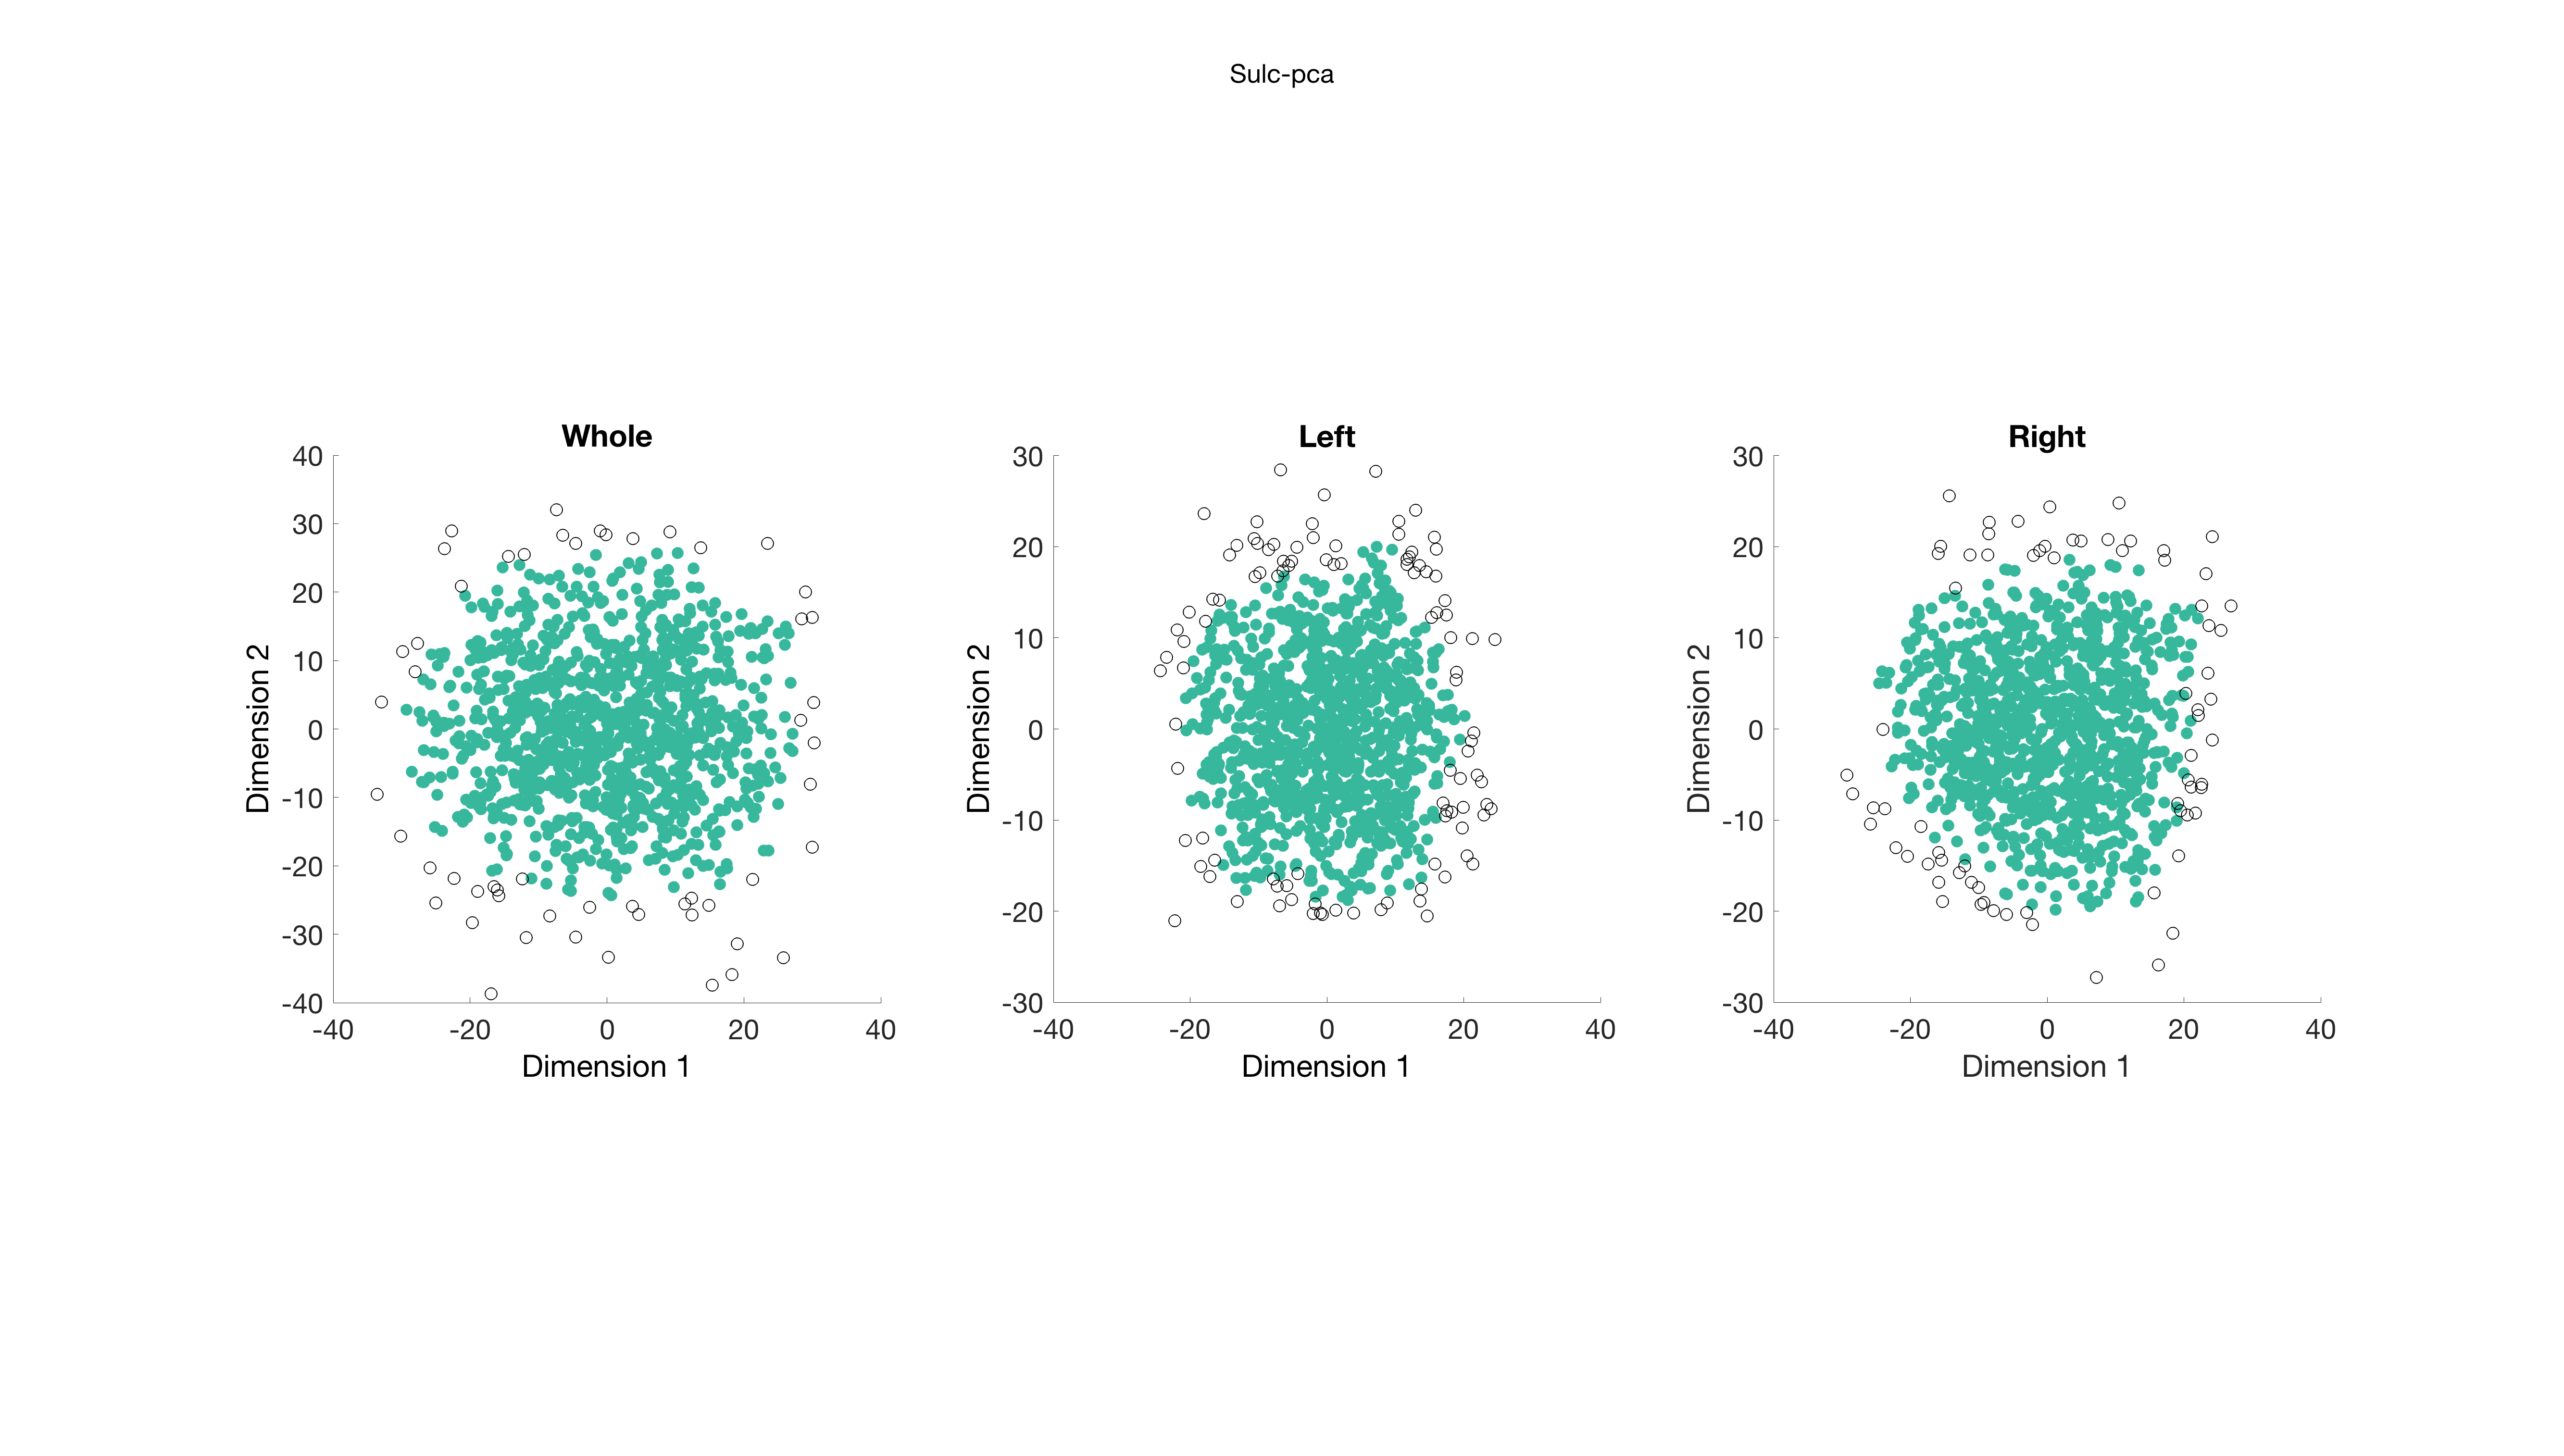
\includegraphics[width=1\textwidth]{LowDReps_Sulc_pca.png}}
\newpage
\section{Thickness Univariate}
\centerline{\includegraphics[width=1.2\textwidth]{Thickness_Univ_Map_Left.png}}
\centerline{\includegraphics[width=1.2\textwidth]{Thickness_Univ_Map_Right.png}}

\newpage
\section{Thickness SVM Left}
\centerline{\includegraphics[width=1.2\textwidth]{ThicknessHistograms_Left.png}}
\centerline{\includegraphics[width=1.2\textwidth]{Thickness_Map_Left.png}}

\newpage
\section{Thickness SVM Right}
\centerline{\includegraphics[width=1.2\textwidth]{ThicknessHistograms_Right.png}}
\centerline{\includegraphics[width=1.2\textwidth]{Thickness_Map_Right.png}}

\newpage
\section{Curvature LIBSVM Left}
\centerline{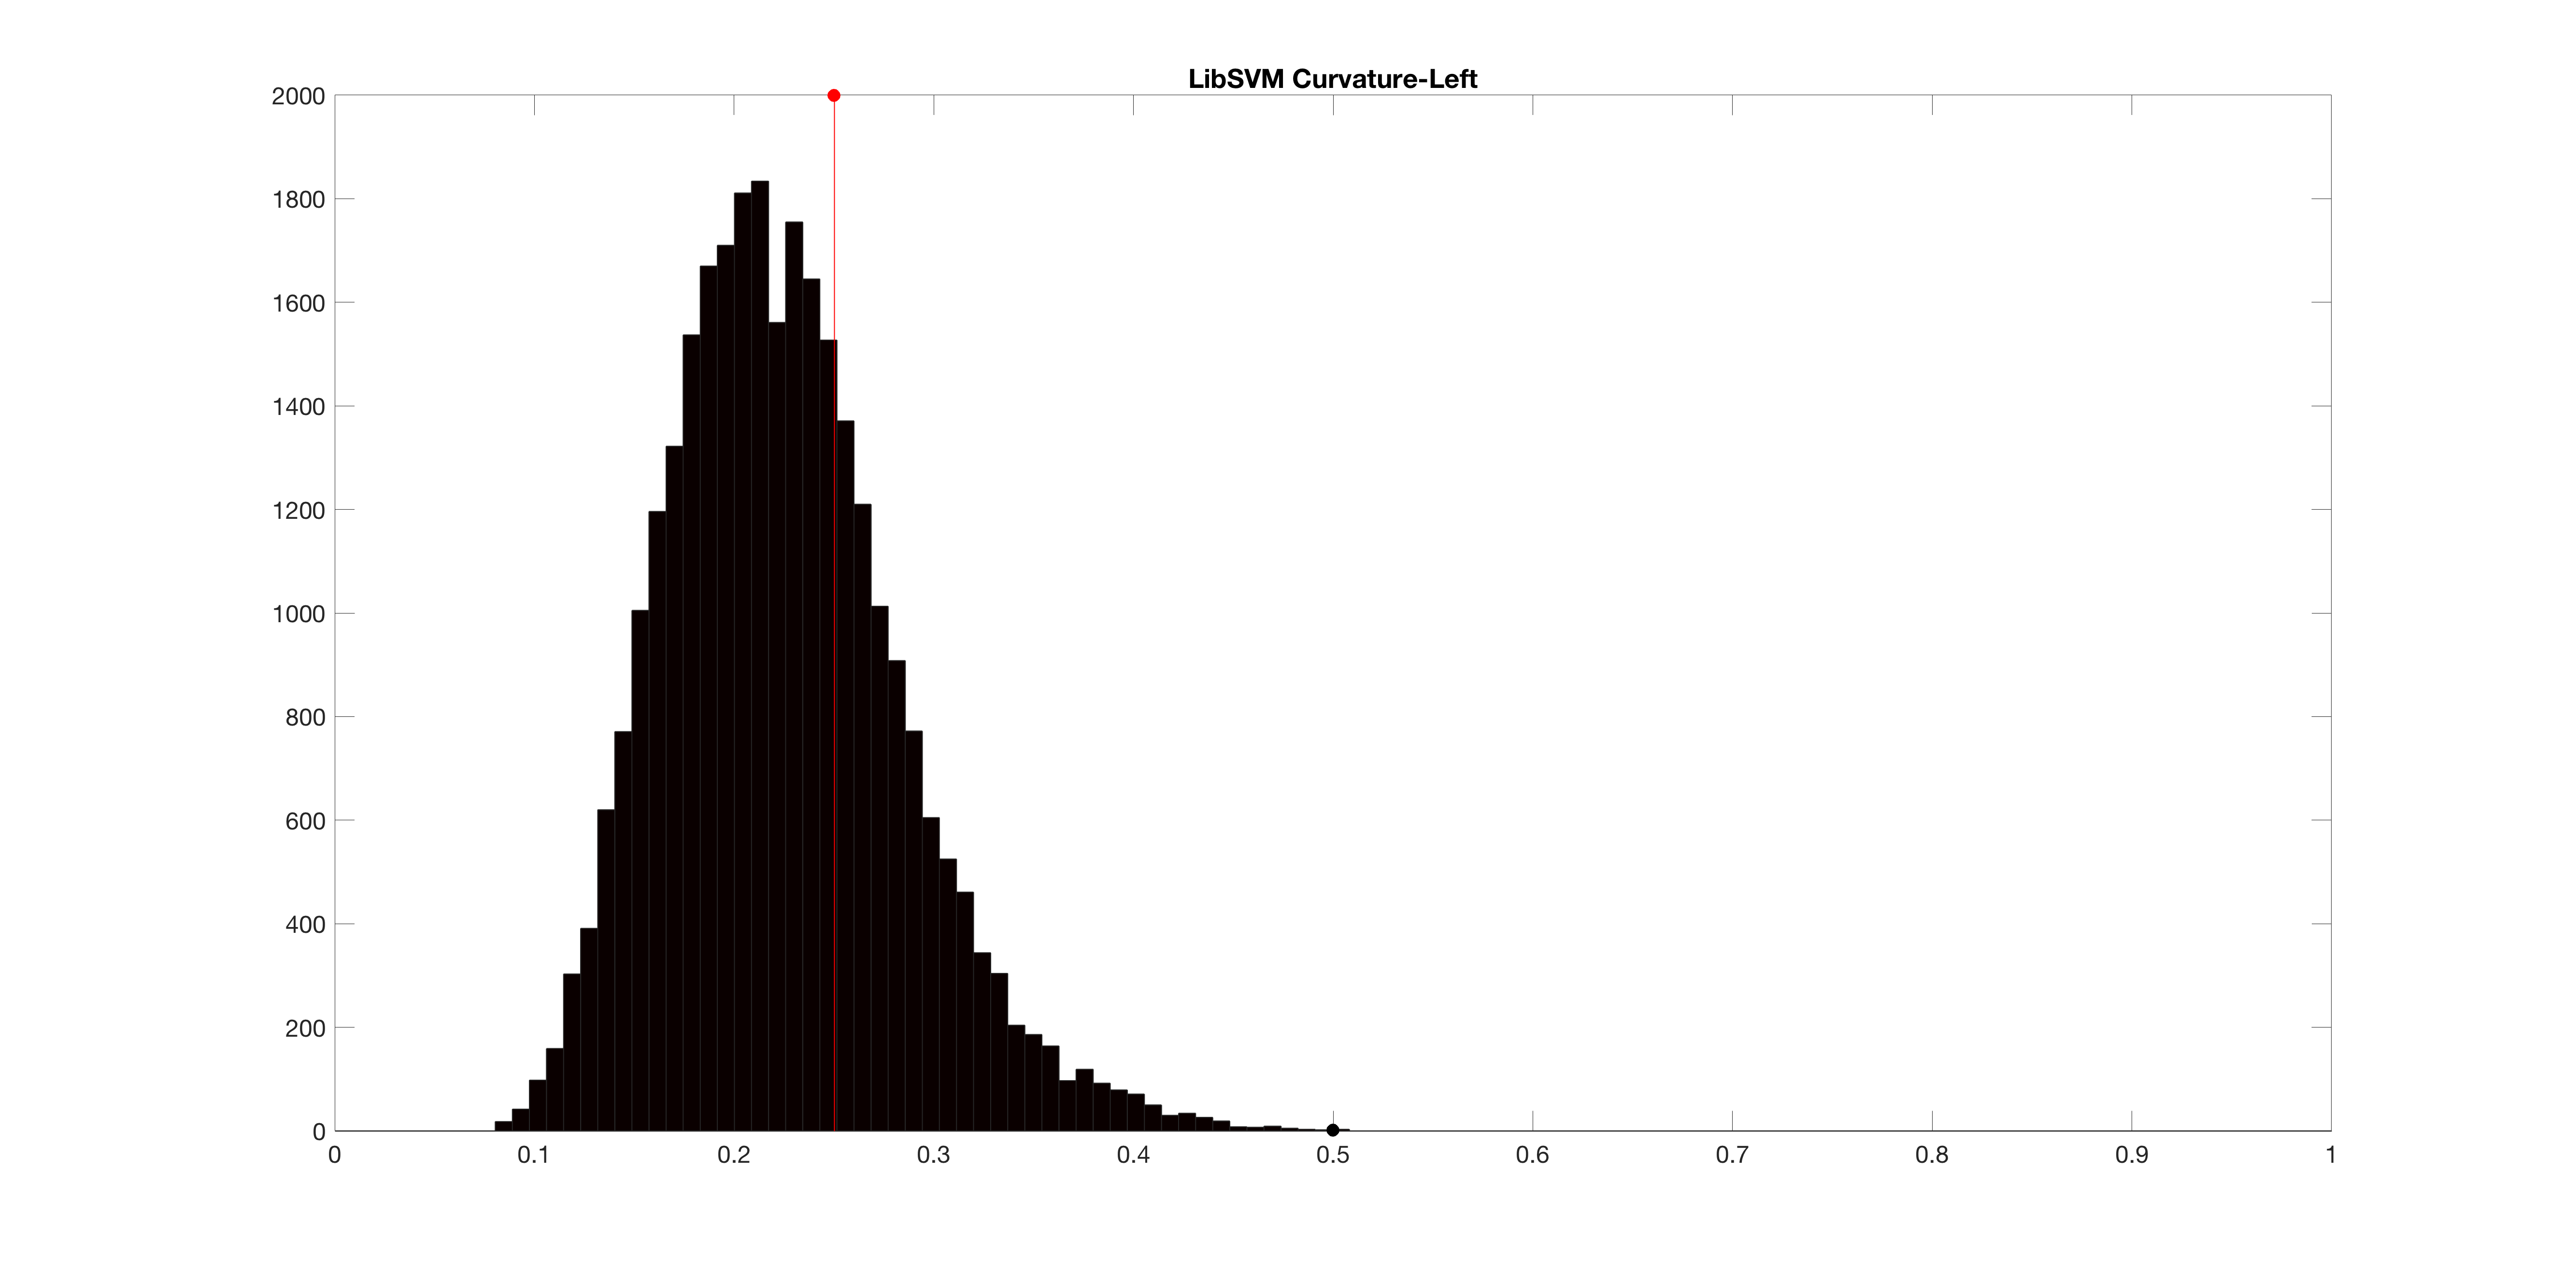
\includegraphics[width=1.2\textwidth]{Curvature_LibSVM_Histograms_Left.png}}
\centerline{\includegraphics[width=1.2\textwidth]{Curvature_LibSVM_Map_Left.png}}
\newpage
\section{Curvature LIBSVM Right}
\centerline{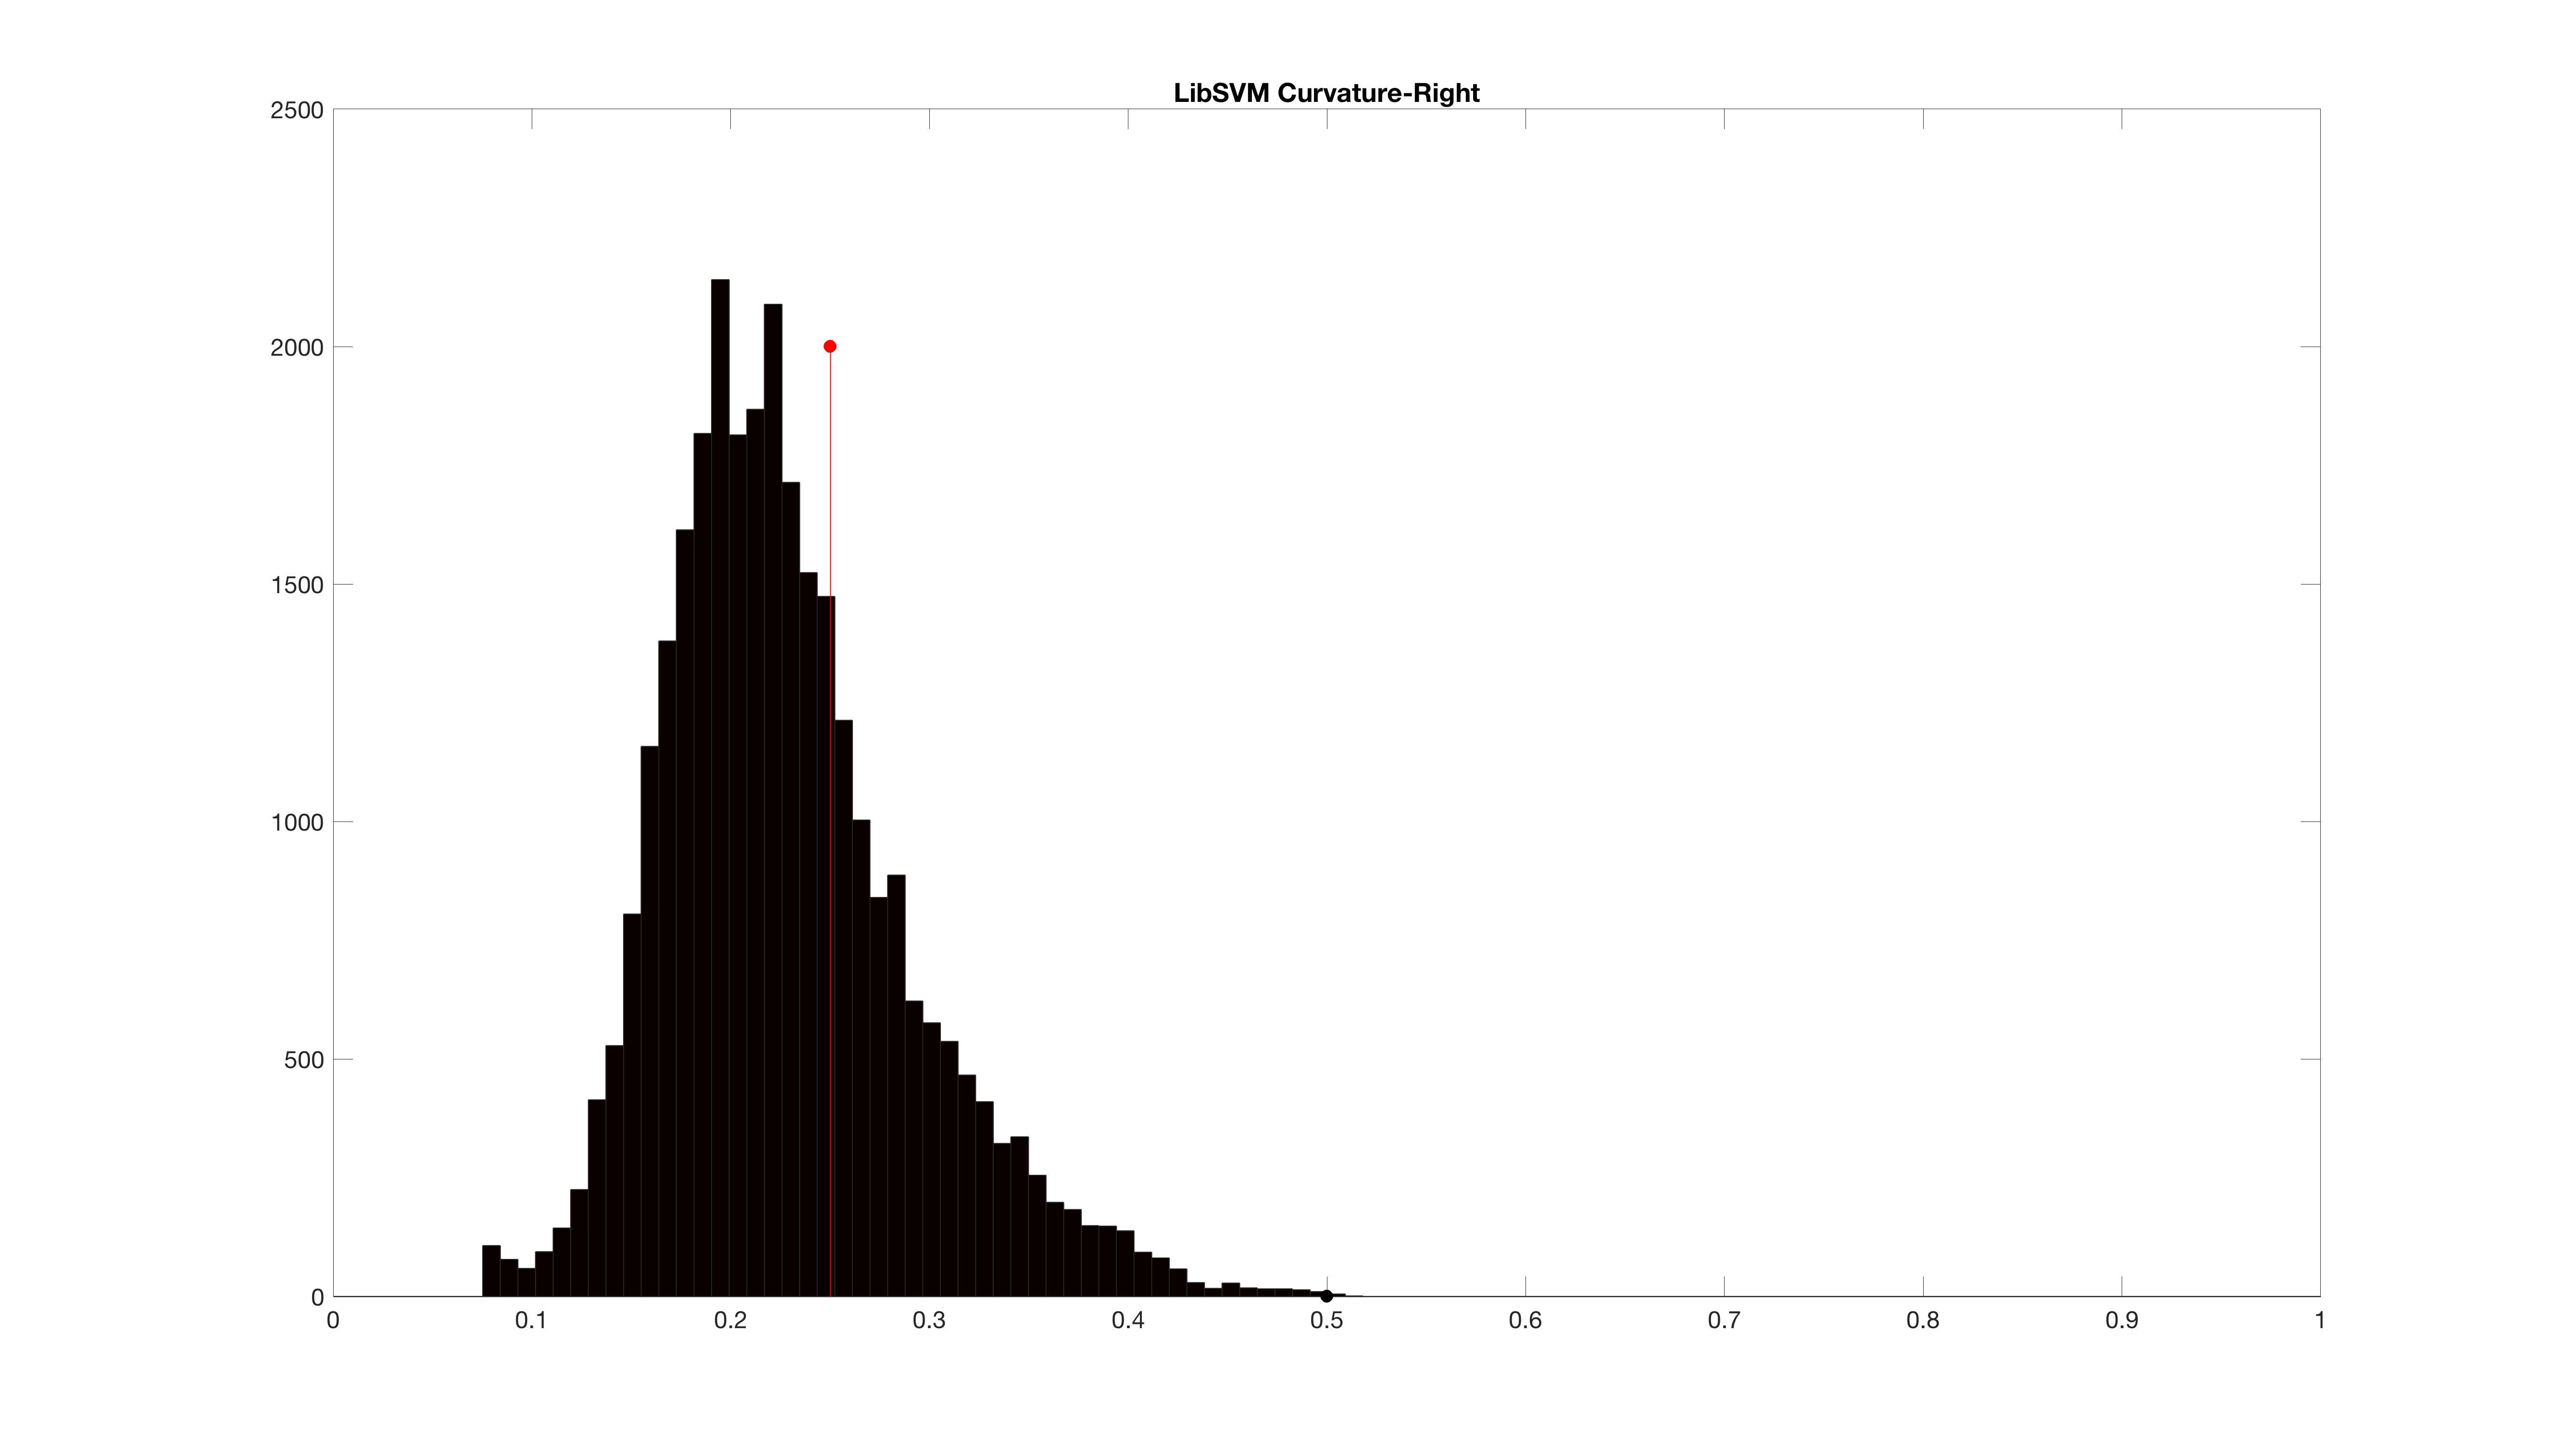
\includegraphics[width=1.2\textwidth]{Curvature_LibSVM_Histograms_Right.png}}
\centerline{\includegraphics[width=1.2\textwidth]{Curvature_LibSVM_Map_Right.png}}


\newpage
\vspace*{-3cm}
\section{Thickess Left RSA}
\centerline{\includegraphics[width=0.8\textwidth]{RSAModels_Thickness_Left.png}}
\centerline{\includegraphics[width=0.8\textwidth]{RSAHists_Thickness_Left.png}}
\centerline{\includegraphics[width=1\textwidth]{RSAMaps_Thickness_Left.png}}

\newpage
\vspace*{-3cm}
\section{Thickess Right RSA}
\centerline{\includegraphics[width=0.8\textwidth]{RSAModels_Thickness_Right.png}}
\centerline{\includegraphics[width=0.8\textwidth]{RSAHists_Thickness_Right.png}}
\centerline{\includegraphics[width=1\textwidth]{RSAMaps_Thickness_Right.png}}

\end{document}
